\chapter{Introduzione}

//TODO la e' non va bene, bisogna usare è

\begin{listing}
    \begin{minted}{Python}
        def hello_world():
            print("Hello floating world!")
    \end{minted}
    \caption{Floating listing.}
    \label{lst:hello}
\end{listing}

\section{Differenze tra relational/non-relational DB}
Lorem ipsum dolor sit amet, consectetur adipiscing elit. Suspendisse et ex vehicula, interdum mi eu, auctor augue. Suspendisse vel sagittis urna. In vitae ligula ipsum. Vivamus mattis neque efficitur, gravida purus facilisis, rhoncus felis. Class aptent taciti sociosqu ad litora torquent per conubia nostra, per inceptos himenaeos. Nunc bibendum urna porta quam congue ornare. Fusce eget consequat libero. Donec varius justo vel libero malesuada, sit amet dignissim ex tincidunt. In pharetra vestibulum lacus quis laoreet. Donec vel laoreet ex, sed facilisis massa. Mauris commodo velit est. Maecenas non sem elementum, faucibus velit et, bibendum mi. Integer laoreet ex et eros accumsan, nec dapibus nisi vestibulum. Donec sed nunc quis mi gravida congue non vel tortor. Interdum et malesuada fames ac ante ipsum primis in faucibus.

Nullam non pharetra arcu. Donec eget velit elit. Pellentesque sed tortor sodales neque tristique rutrum. Vivamus et ex dolor. Vestibulum lacinia augue sit amet libero mattis pellentesque. In sed congue ante, quis tempus neque. Vestibulum semper eu sapien et vestibulum.

In ac erat ullamcorper, ultricies dolor sit amet, tempus neque. Pellentesque quam erat, ornare ac justo at, cursus luctus ex. Pellentesque at turpis blandit, elementum ex ac, fringilla nibh. Etiam et tincidunt lacus. Integer mattis mi sit amet faucibus rutrum. Sed at nisi commodo, ultricies purus a, tempus lacus. Mauris accumsan enim nisi, in tempor velit pharetra eu. Sed eu turpis et ante sagittis sodales. Duis a tellus id risus ultricies accumsan. Vestibulum bibendum in sapien sit amet rhoncus. Fusce aliquam, metus vel efficitur pulvinar, nibh lacus ultricies nisl, nec rhoncus elit ligula vitae risus. Mauris bibendum eget erat non rutrum. Curabitur in ligula eget lectus facilisis molestie sed sed neque. Vestibulum eu faucibus augue, a luctus augue. Nam lobortis massa non lorem condimentum vehicula. Aliquam efficitur cursus neque, efficitur placerat libero tincidunt non. Nullam.

\section{Il nostro caso di studio}

Durante la progettazione si e' deciso di utilizzare una relazione per poter testare i diversi metodi di collezione dei dati.
La relazione e' formata da 2 entita' A e B,in un esempio di un social network l'entita' A sono i Post e l'entita' B i Commenti sotto ogni post, collegate da una relazione 1..N -> 1...1,
per ogni A esistono 10 B relativi, ogni Post contiene 10 Commenti.

La modellazione delle entita' e' stata fatta creando 2 triplette di attributi uguali, sulla seconda tripletta al contrario della prima sono stati costruiti degli indici su ogni attributo,
questi attributi generici hanno una propria selettivita':

    \begin{equation*}
        \left.\begin{aligned}
         sel(Att1, Att4) &= \frac{1}{10}    \\
         sel(Att2, Att5) &= \frac{1}{10.000} \\
         sel(Att2, Att6) &= \frac{1}{100}
        \end{aligned}
        \right\}
        \qquad 
        \end{equation*}

Poi un attributo testaule, A7, di 100 bytes per poter inserire descrizione.

Il numero di Entita' A e' di $10^5$ e di conseguenza ci sono $10^6$ entita' B.

\fvset{gobble=2}
\begin{Verbatim}[frame=single,framesep=2mm,label=A (POST),labelposition=all]
{
  "_id": 6808,
  "AK": 6808,
  "A1": 3042,
  "A2": 300,
  "A3": 8,
  "A4": 3042,
  "A5": 300,
  "A6": 8,
  "A7": "Lorem ipsum dolor sit amet, consectetur adipiscing elit. 
    Fusce lacinia eget arcu et maximus. Ut tempus est sit amet 
    tortor commodo, sit amet facilisis mi rhoncus. Donec et elit
    venenatis, consequat tellus eu, tristique orci. Duis 
    tristique sem ut nulla ullamcorper, a porta risus efficitur.
    Cras sed neque et nisl tincidunt vestibulum. Phasellus 
    tristique tempor facilisis. Sed facilisis lectus eros, sed 
    aliquet lacus elementum sed. Integer vel dictum mi. 
    Maecenas pharetra tempus eros, efficitur mattis erat cursus
    in. Nulla sit amet quam velit. Nullam tempus dictum lacus
    id porttitor. Vestibulum facilisis pulvinar fermentum.
    Ut elementum maximus feugiat. In at mollis leo, eu 
    facilisis magna. Vestibulum sed nisi ultricies, tincidunt
    enim ac, fringilla ex. Phasellus pharetra mollis nisi
    a fermentum. In nec faucibus nulla, eget molestie magna.
    Vivamus in gravida ex. Aenean scelerisque gravida 
    ipsum, nec congue enim posuere sit amet. Donec vitae felis
    id sem congue blandit eget non justo quis."
}
\end{Verbatim}

% \begin{minted}{js}
% {
%   "_id": 6808,
%   "AK": 6808,
%   "A1": 3042,
%   "A2": 300,
%   "A3": 8,
%   "A4": 3042,
%   "A5": 300,
%   "A6": 8,
%   "A7": 'Lorem ipsum dolor sit amet, consectetur adipiscing elit.' 
%     'Fusce lacinia eget arcu et maximus. Ut tempus est sit amet'  
%     'tortor commodo, sit amet facilisis mi rhoncus. Donec et elit'
%     'venenatis, consequat tellus eu, tristique orci. Duis'
%     'tristique sem ut nulla ullamcorper, a porta risus efficitur.'
%     'Cras sed neque et nisl tincidunt vestibulum. Phasellus' 
%     'tristique tempor facilisis. Sed facilisis lectus eros, sed' 
%     'aliquet lacus elementum sed. Integer vel dictum mi.'
%     'Maecenas pharetra tempus eros, efficitur mattis erat cursus'
%     'in. Nulla sit amet quam velit. Nullam tempus dictum lacus'
%     'id porttitor. Vestibulum facilisis pulvinar fermentum.'
%     'Ut elementum maximus feugiat. In at mollis leo, eu'
%     'facilisis magna. Vestibulum sed nisi ultricies, tincidunt'
%     'enim ac, fringilla ex. Phasellus pharetra mollis nisi' 
%     'a fermentum. In nec faucibus nulla, eget molestie magna.'
%     'Vivamus in gravida ex. Aenean scelerisque gravida'
%     'ipsum, nec congue enim posuere sit amet. Donec vitae felis'
%     'id sem congue blandit eget non justo quis' 
% }
% \end{minted}
% 
% \begin{minted}[]{js}
%     
% {
%   "_id": 73888,
%   "BK": 738878,
%   "F_AK": 70394,
%   "B1": 94207,
%   "B2": 176,
%   "B3": 3,
%   "B4": 94207,
%   "B5": 176,
%   "B6": 3,
%   "B7": 'Lorem ipsum dolor sit amet, consectetur adipiscing elit.' 
%     'Fusce lacinia eget arcu et maximus. Ut tempus est sit amet'  
%     'tortor commodo, sit amet facilisis mi rhoncus. Donec et elit'
%     'venenatis, consequat tellus eu, tristique orci. Duis'
%     'tristique sem ut nulla ullamcorper, a porta risus efficitur.'
%     'Cras sed neque et nisl tincidunt vestibulum. Phasellus' 
%     'tristique tempor facilisis. Sed facilisis lectus eros, sed' 
%     'aliquet lacus elementum sed. Integer vel dictum mi.'
%     'Maecenas pharetra tempus eros, efficitur mattis erat cursus'
%     'in. Nulla sit amet quam velit. Nullam tempus dictum lacus'
%     'id porttitor. Vestibulum facilisis pulvinar fermentum.'
%     'Ut elementum maximus feugiat. In at mollis leo, eu'
%     'facilisis magna. Vestibulum sed nisi ultricies, tincidunt'
%     'enim ac, fringilla ex. Phasellus pharetra mollis nisi' 
%     'a fermentum. In nec faucibus nulla, eget molestie magna.'
%     'Vivamus in gravida ex. Aenean scelerisque gravida'
%     'ipsum, nec congue enim posuere sit amet. Donec vitae felis'
%     'id sem congue blandit eget non justo quis' 
% }
% \end{minted}

    !!!!!!!!!! LE FOTO NON VANNO BENE, LE CHIAVI DEVONO ESSERE SEGNALATE !!!!!!!!!!!!!!!!!!!!!!!!!
\begin{center}
    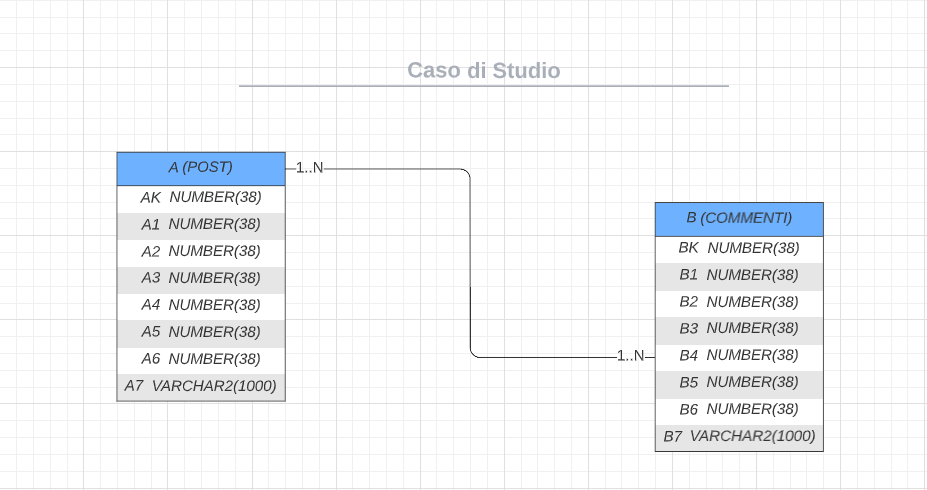
\includegraphics[scale=0.6]{Caso Studio.png}
\end{center}


\section{Modellazione dei dati}

La modellazione dei dati ha un ruolo fondamentale nel calcolo dei costi di accesso e quindi costi di esecuzione delle query, le soluzioni dalle quali si e' deciso di di partire 
sono quelle dell'Embedding e del Referencing. Utilizzando un sistema non relazionale abbiamo necessita' di esprimere la relazione tra A e B in un modo differente, attraverso il 
referencing colleghiamo le un entita' inserendo un riferimento della seconda e viceversa, per poter poi eseguire ad esempio query di join o voler recuperare tutti i dati 
dell'entita' referenziata c'e' il bisogno di mantenere all'interno del database la collezione contenente i rimanenti attributi. Es. nell'eventuale soluzione del referencing di B all'interno 
di A, ci sono due collezioni ossia A con la foreign key relativa (BK) relativa a B e l'intera collezione B. 

//TODO cambiare assolutamente queste foto
\begin{center}
    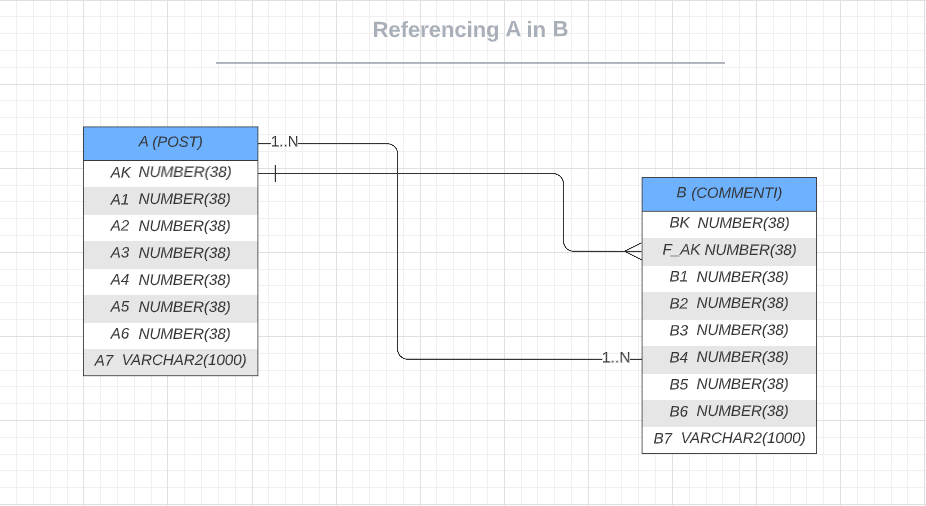
\includegraphics[scale=0.6]{refAB.png}
\end{center}

\begin{center}
    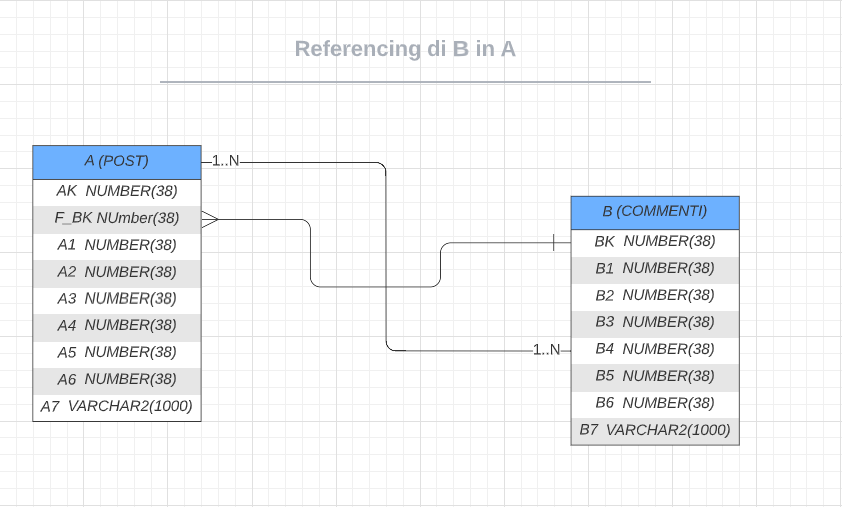
\includegraphics[scale=0.6]{refBA.png}
\end{center}

La soluzione embedding consiste nel creare un'unica collezione di documenti che racchiudono al loro interno sia documenti di A che documenti di B.

\begin{center}
    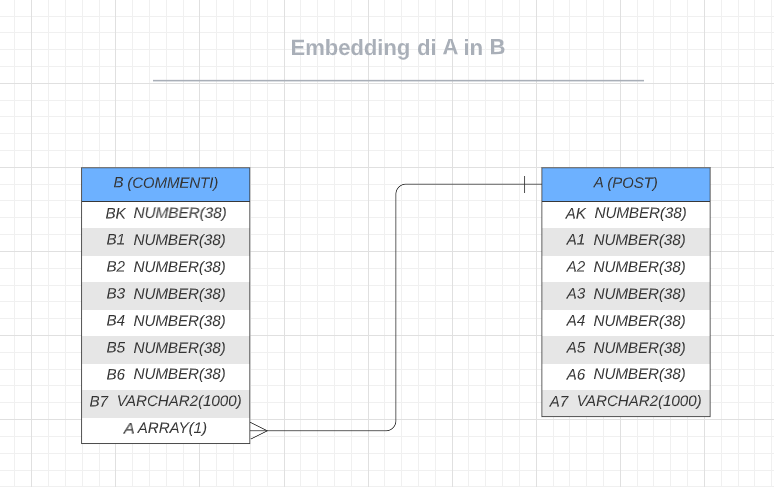
\includegraphics[scale=0.6]{embAB.png}
\end{center}

\begin{center}
    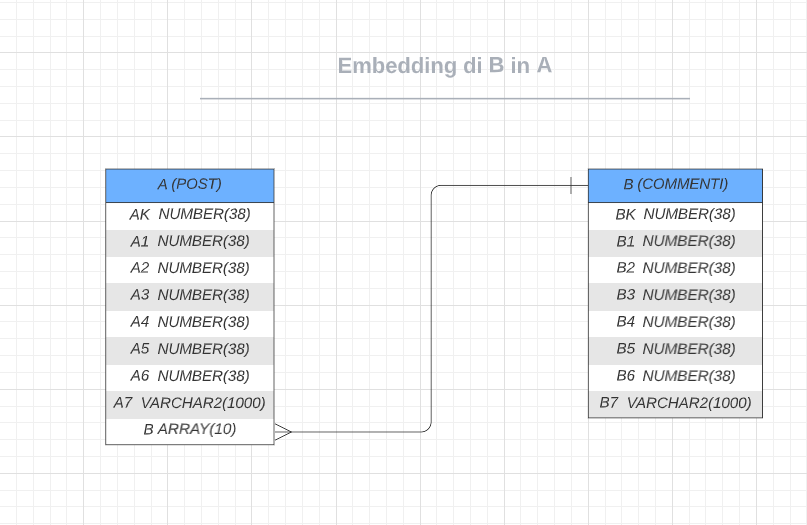
\includegraphics[scale=0.6]{embBA.png}
\end{center}

//TODO section che spiega le operanzioni CRUD

//TODO section che spiega le query  che verranno effettuate sulle collezioni di dati (selezione e update)

\section{Query e operazioni}

Per poter ottenere statistiche da ogni database, sono state decise delle query legate alle operazioni CRUD.

Le prime ad essere eseguite sono state quelle di \textbf{inserimento} di dati, i cui risultati si trovano rispettivamente nelle sezioni
\begin{itemize}
    \item \hyperref[sec:InsertMongo]{Insertimento per MongoDB}
\end{itemize} 

//TODO inserire un grafico con i tempi non sarebbe male

Le query di \textbf{lettura} invece sono le query su cui si è lavorato maggiormente, è stata testata la lettura di ogni attributo di entrambe le 
entità, sia indicizzati che non, escludendo l'attributo di tipo testuale x7 che serve per poter conservare una descrizione del Post o del Commento.

\begin{minted}[]{sql}
    select A.*
    from A
    where Ax='val'
    
    
    select B.*
    from B
    where Bx='val' 
\end{minted}

Data la relazione tra A e B, sono state eseguite poi delle query di selezione di entrambi gli oggetti di una relazione dopo avere eseguito un join 
sulle chiavi primarie e leggendo un particolare valore degli attributi.

\begin{minted}[]{sql}
    select A.*, B.*
    from A join B on (A.AK=B.AK)
    where Ax='val'


    select A.*, B.*
    from A join B on (A.AK=B.BK)
    where Bx='val'
\end{minted}

I valori letti all'interno delle query sono valori randomizzati, ottenuti tramite le cardinalità delle entità, propri per ciascun attributo, in Python con 
ad esempio la seguente funzioni che prende in entrata l'indice sulla quale cercare e ne restituisce un numero valido.

\begin{minted}[]{python}
    expA = 5

    expB = 6

    N_A = 10**expA 

    N_B = 10**expB

    N_A1 = N_A/10

    N_A2 = N_A/10**(round(expA/2))

    N_A3 = N_A/10**(expA - 1)

    N_B1 = N_B/10

    N_B2 = N_B/10**(round(expB/2))

    N_B3 = N_B/10**(expB - 1)

     def get_random_indexed_int_A(ind):
      if "1" in ind or "4" in ind :
        return randint(0, N_A1 - 1)
      elif "2" in ind or "5" in ind:
        return randint(0, N_A2 - 1)
      elif "3" in ind or "6" in ind:
        return randint(0, N_A3 - 1)

    def get_random_indexed_int_B(ind):
      if "1" in ind or "4" in ind :
        return randint(0, N_B1 - 1)
      elif "2" in ind or "5" in ind:
        return randint(0, N_B2 - 1)
      elif "3" in ind or "6" in ind:
        return randint(0, N_B3 - 1)   
\end{minted}

Le query di \textbf{update} sono state strutturate in modo abbastanza simile a quelle di letttura

\begin{minted}[]{sql}
    update A
    set Ay = 'val'
    where Ax='val'

    update B
    set By = 'v'
    where Bx='val'
\end{minted}

//TODO inserire come ho creato i dataset /generazione File 

//TODO valutare se queste section di inserimento sarebbero meglio all interno dei propri capitoli

% \section{Risultati inserimento dati}
% 
% Dopo la creazione dei dataset delle entità A e B, di diverse dimensioni, sono stati verificati i tempi di inserimento per ogni software utilizzato, 
% ognuno utilizza un differente metodo per la creazione di un documento.
